%! Author = borisdeletic
%! Date = 07/05/2023

% Preamble
\documentclass[11pt]{article}

% Document
\begin{document}


\section{Lattice Field Theory}\label{sec:LFT}

\subsection{Laattice Field Theory for Markov-Chain Monte Carlo methods}\label{subsec:lft_mcmc}
    The path integral formalism for quantum mechanics provides a powerful tool for studying relativistic
    quantum field theories~\cite{Feynman1948}.
    It is written as a functional integral
    \begin{equation}\label{eq:path_integral}
    \mathcal{Z} = \int {\mathcal{D}\phi e^{iS[\phi]}},
    \end{equation}
    where $\mathcal{D}\phi$ is a measure over all field configurations $\phi$, and $e^{iS[\phi]}$ weights the contribution
    of each configuration.
    In the classical limit, all the `unphysical` fields with very a large action cancel each other, and we reduce
    to Hamilton's least action principle.

    The path integral approach provides a useful starting point for lattice field theory.
    We begin by discretizing space-time, such that the field $\phi(x)$ lives on a finite lattice rather than in a
    continuous space.
    However, this still leaves a sum over an infinite number of possible field configurations.
    In order to computationally measure observables of a field theory system, we must employ MCMC methods to estimate
    the path integral.

    In order to interpret the field weight factor $e^{iS[\phi]}$ as a probability for a given configuration,
    we can perform a Wick-rotation by redefining time as imaginary~\cite{rothe2005lattice}.
    \begin{equation}\label{eq:wick_rotation}
    \begin{aligned}
        t &\rightarrow i \tau, \\
        $e^{iS[\phi]}$ &\rightarrow e^{-S_E[\phi]},
    \end{aligned}
    \end{equation}
    where from now on we only refer to the Euclidean action as $S$.

    This factor is now a well-defined probability distribution as it is bounded and normalised
    $P[\phi] \equiv \frac{1}{Z} e^{-S[\phi]} > 0$.
    Therefore, it is possible to apply MCMC methods to sample from this distribution and calculate observables
    with an acceptance probability
    \begin{equation}\label{eq:accept_prob_lft}
    \begin{aligned}
        A(\phi'|\phi) = \min \left(1, \frac{\exp(-S[\phi'])}{\exp(-S[\phi])} \right),
    \end{aligned}
    \end{equation}

\subsection{Scalar $\phi^4$ Theory}\label{subsec:phi^4_theory}
    We work with a real, scalar $\phi^4$-theory in two-dimensions, discretized to a Euclidean square lattice of length $N$.
    The dimensionless action for the theory is given by
    \begin{equation}\label{eq:phi4_action}
    \begin{aligned}
        S = \,\sum\limits_{x \in \Lambda} \Biggl[-2\kappa \sum\limits_{\mu=1}^d & \phi(x) \phi(x+\hat{\mu}) \\
        &+\lambda \phi(x)^4 + (1 - 2\lambda) \phi(x)^2 \Biggr],
    \end{aligned}
    \end{equation}
    where $\Lambda$ is the set of lattice points, $\hat{\mu}$ is the unit vector in $\mu$ direction, and $\phi(x)$ is
    the field value at lattice site $x$~\cite{maas2020lattice}. $\kappa$ is the kinetic coupling for neighbour interactions and $\lambda$ is the
    coupling strength of the interaction.

    $\phi^4$ theory lives in the same universality class as the 2D Ising model, and we recover the Ising model
    in the limit $\lambda \rightarrow \infty$.
    As such, the model exhibits a second-order phase transition in the $\kappa, \lambda$ parameters, associated
    with the breaking of $\mathcal{Z}_2$ symmetry.

    The order parameter which undergoes a phase transition is the mean magnetization, defined as the normalised
    expectation of absolute field value
    \begin{equation}\label{eq:magnetization}
        \langle M \rangle = \frac{1}{N^2} \bigl< \sum_{x \in \Lambda} |\phi(x)| \bigr>.
    \end{equation}


\subsection{Nested Sampling for $\phi^4$ Theory}\label{subsec:nested-sampling-phi4}
    As described in~\ref{subsec:lft_mcmc}, we sample from the distribution with probability $P[\phi] = e^{-S[\phi]}$.
    Therefore, defining the log likelihood function as $\log{\mathcal{L}} = -S[\phi]$ the problem is reframed in
    Bayesian inference terms, allowing us to apply the new algorithm we have introduced in~\ref{sec:chmc}.

    The model of $\phi^4$-theory is a good candidate to test CHMC for nested sampling for a number of reasons.
    Below the critical point, the loglikelihood is a bimodal distribution allowing us to investigate the clustering
    behaviour of the algorithm.
    The likelihood gradient is also analytic
    \begin{equation}\label{eq:grad_likelihood}
    \begin{aligned}
        \frac{\partial \log{\mathcal{L}}} {\partial \phi(x)} = -2\kappa \sum\limits_{\mu} &\phi(x+\hat{\mu}) \\
        &+ 4\lambda \phi(x)^3 + 2(1-2\lambda)\phi(x)
    \end{aligned}
    \end{equation}
    and well-behaved.
    Furthermore, as we approach the critical point, this model exhibits \emph{critical slowing down}, allowing us to
    test the algorithm's resilience to this phenomenon.

    \begin{figure}[t!]
        \centering
        \begin{subfigure}{\linewidth}
            \centering
            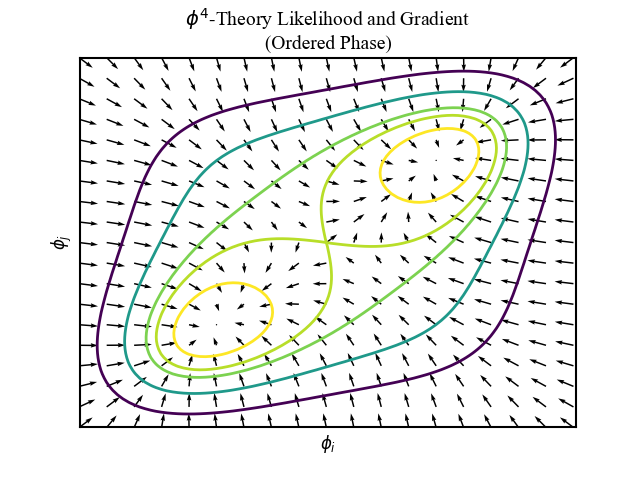
\includegraphics[width=\linewidth]{../figures/Phi4LikelihoodOrdered}
            \caption{
            In the ordered phase, neighbouring fields prefer aligning in the same direction as each other.
            This results in a bimodal distribution with a positive mean magnetisation $\langle M \rangle$.}
            \label{fig:phi4likelihood_ordered}
        \end{subfigure}
        \begin{subfigure}{\linewidth}
            \centering
            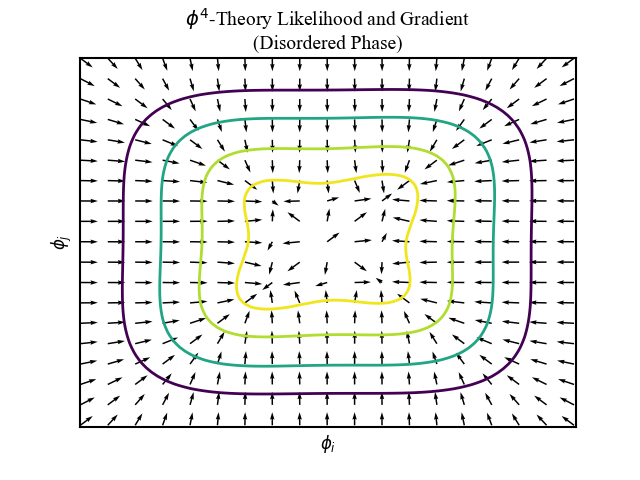
\includegraphics[width=\linewidth]{../figures/Phi4LikelihoodDisordered}
            \caption{
            In the disordered phase, neighbouring fields are uncorrelated. The likelihood is a unimodal distribution
            with zero mean magnetisation $\langle M \rangle$.}
            \label{fig:phi4likelihood_disordered}
        \end{subfigure}
    \end{figure}

    When using CHMC and nested sampling for $\phi^4$ theory, we must define a prior distribution $\pi(\theta)$.
    To use CHMC, we already provide the likelihood function gradient for reflections.
    Therefore, we can set the prior to be the posterior by using the likelihood function as the
    prior $\pi(\theta) = \mathcal{L}(\theta)$.
    This removes the need for any new gradients and maximises the speed of convergence, as sampling directly from the
    posterior will be most efficient.


\end{document}